% *******************************************************************************
% * Copyright (c) 2007 by Elexis
% * All rights reserved. This document and the accompanying materials
% * are made available under the terms of the Eclipse Public License v1.0
% * which accompanies this distribution, and is available at
% * http://www.eclipse.org/legal/epl-v10.html
% *
% * Contributors:
% *    G. Weirich - initial implementation
% *
% *  $Id: einleitung.tex 4904 2009-01-03 17:58:33Z rgw_ch $
% *******************************************************************************
% !Mode:: "TeX:UTF-8" (encoding info for WinEdt)

\section{Einleitung}
Für das Erstellen von Briefen, Rezepten, Zeugnissen etc. greift Elexis
standardmässig auf ein vollwertiges Büroprogramm zurück: OpenOffice.

Dies muss zwar nicht zwingend so sein, da das Textsystem von Elexis als Plugin
ausgeführt wird. Man könnte also auch ein Plugin erstellen (lassen), das
Microsoft\texttrademark{}Office\texttrademark{} oder irgendein anderes Textsystem
benutzt. Wir möchten hier aber nur auf das standardmässig verwendete OpenOffice
eingehen.

OpenOffice.org geht auf das in den 80er Jahren entwickelte StarOffice zurück und
ist heute eine Office-Suite analog zu Microsoft Office, mit dem Unterschied,
dass es quelloffen und für mehrere Betriebssysteme erhältlich ist.

Im Installer der Windows-Version von Elexis ist bereits eine geeignete OpenOffice.org Version integriert. Bei Linux kann man in der Regel auf die OpenOffice-Version zurückgreifen, die standardmässig bei Linux eingeschlossen ist. Beim Macintosh funktioniert die Integration leider noch nicht.
Beachten Sie, dass nur eine OpenOffice-Version im System installiert sein sollte. Andernfalls kann es Konflikte zwischen den Versionen geben.

\medskip

Nach der Installation von OpenOffice und Elexis müssen Sie die beiden Programme
noch miteinander bekannt machen. Dies geschieht innerhalb von Elexis, indem Sie
das Textplugin so konfigurieren, dass es auf OpenOffice zugreift (Das Plugin
\glqq NOA-Text\footnote{Wir verwenden das Modul 'Nice Office Access' von \href{http://www.ubion.org}{www.ubion.org}
 zum Einbinden von OpenOffice}\grqq{}muss hierzu installiert sein, was standardmässig der Fall ist.

Wählen Sie im Menu \textsc{Datei - Einstellungen - Textverarbeitung}
Es erscheint eine Dialogbox wie in Abb \ref{fig:text1}. Wählen Sie dort \glqq
%\usepackage{graphics} is needed for \includegraphics
\begin{figure}[htp]
\begin{center}
  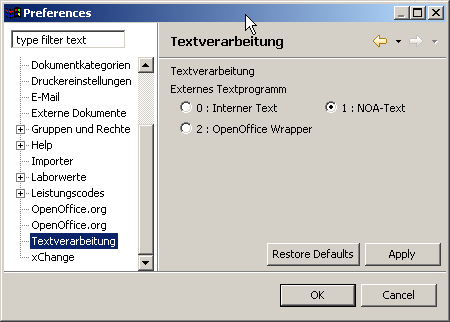
\includegraphics{images/text1}
  \caption{Konfiguration des Textplugins}
  \label{fig:text1}
\end{center}
\end{figure}

NOA-Text\grqq{}. Gehen Sie dann zum Feld OpenOffice.org (S. Abb. \ref{fig:text2}
und wählen Sie durch Klick auf \glqq definieren\grqq{}den Pfad zu Ihrer
OpenOffice-Installation aus.
%\usepackage{graphics} is needed for \includegraphics
\begin{figure}[htp]
\begin{center}
  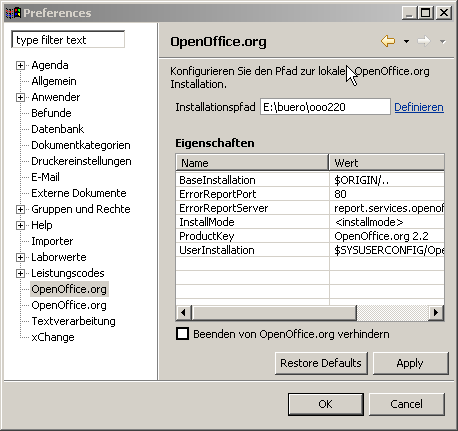
\includegraphics{images/text2}
  \caption{Konfiguration der OpenOffice-Installation}
  \label{fig:text2}
\end{center}
\end{figure}
Ab dem, nächsten Start von Elexis sollte OpenOffice dann zur Verfügung stehen
(Bei der ersten Verwendung werden Sie noch den Lizenzbedingungen von
OpenOffice.org zustimmen müssen)



